\chapter{Caso Real}
\label{ch:caso_real}

\textbf{Ejemplo 1.}
$\langle p(t),q(t) \rangle_{\textbf{M}_S}=\int_{-1}^{1} p(t)q(t)t^2 \, dt + \int_{-1}^{1} p'(t)q'(t)t^{10} \, dt $

\begin{center}
	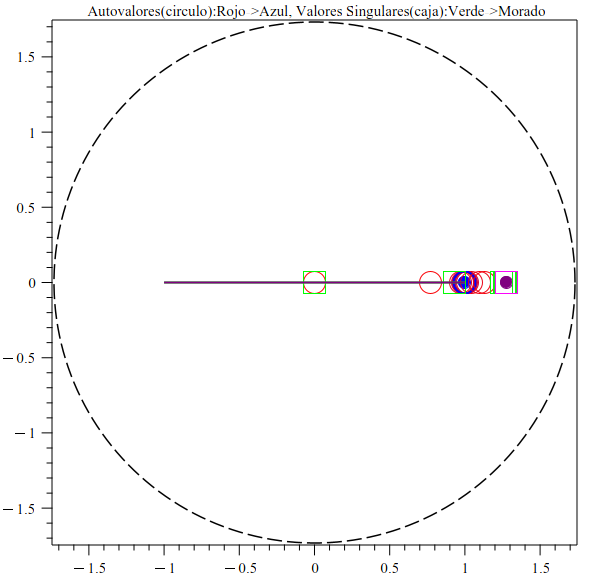
\includegraphics[width=0.9\textwidth]{include/a-1b1t2t10.png}
\end{center}

\begin{enumerate}
	\item $\lim_{n \to 50}\sigma_{1,n}=1.276$
	\item $\lim_{n \to 50} \rho(\mathcal{D}_{n})=0.999$
	\item $\max\{\rho(\mathcal{D}_{n})\}_{n=0}^{50}=1.133$
	\item $\lim_{n \to 50}\sigma_{2,n}$ no disponible
\end{enumerate}

\textbf{Ejemplo 2.}
$\langle p(t),q(t) \rangle_{\textbf{M}_S}=\int_{-1}^{1} p(t)q(t)t^{10} \, dt + \int_{-1}^{1} p'(t)q'(t)t^{2} \, dt $

\begin{center}
	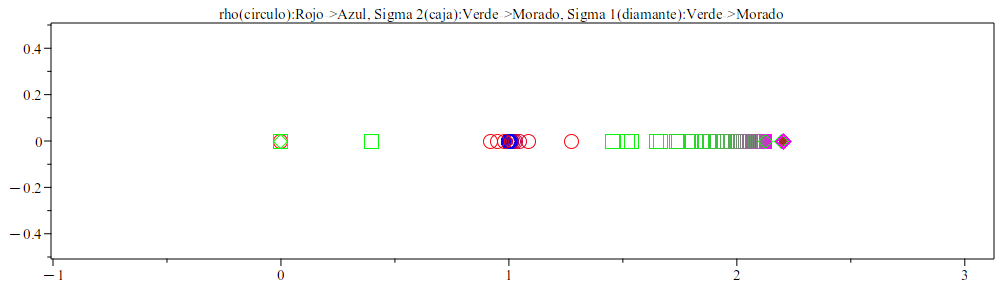
\includegraphics[width=0.9\textwidth]{include/a-1b1t10t2.png}
\end{center}

\begin{enumerate}
	\item $\lim_{n \to 50}\sigma_{1,n}=2.204$
	\item $\lim_{n \to 50} \rho(\mathcal{D}_{n})=0.999$
	\item $\max\{\rho(\mathcal{D}_{n})\}_{n=0}^{50}=1.275$
	\item $\lim_{n \to 50}\sigma_{2,n}$ no disponible
\end{enumerate}


\textbf{Ejemplo 3.}
$\langle p(t),q(t) \rangle_{\textbf{M}_S}=\int_{0}^{10} p(t)q(t) \, dt + \int_{30}^{40} p'(t)q'(t) \, dt $

\begin{center}
	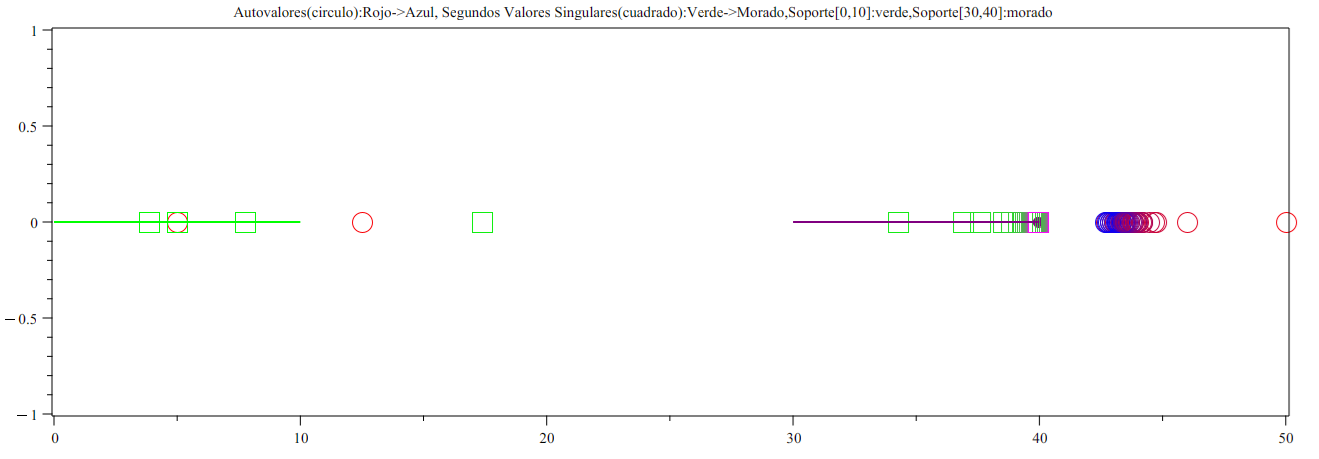
\includegraphics[width=1\textwidth]{include/a0b10c30d40.png}
\end{center}

\begin{enumerate}
	\item $\lim_{n \to 50}\sigma_{1,n}=\infty$
	\item $\lim_{n \to 50} \rho(\mathcal{D}_{n})=43.133$
	\item $\max\{\rho(\mathcal{D}_{n})\}_{n=0}^{50}=50.052$
	\item $\lim_{n \to 50}\sigma_{2,n}=39.975$
\end{enumerate}

\textbf{Ejemplo 4.}
$\langle p(t),q(t) \rangle_{\textbf{M}_S}=\int_{30}^{40} p(t)q(t) \, dt + \int_{0}^{10} p'(t)q'(t) \, dt $

\begin{center}
	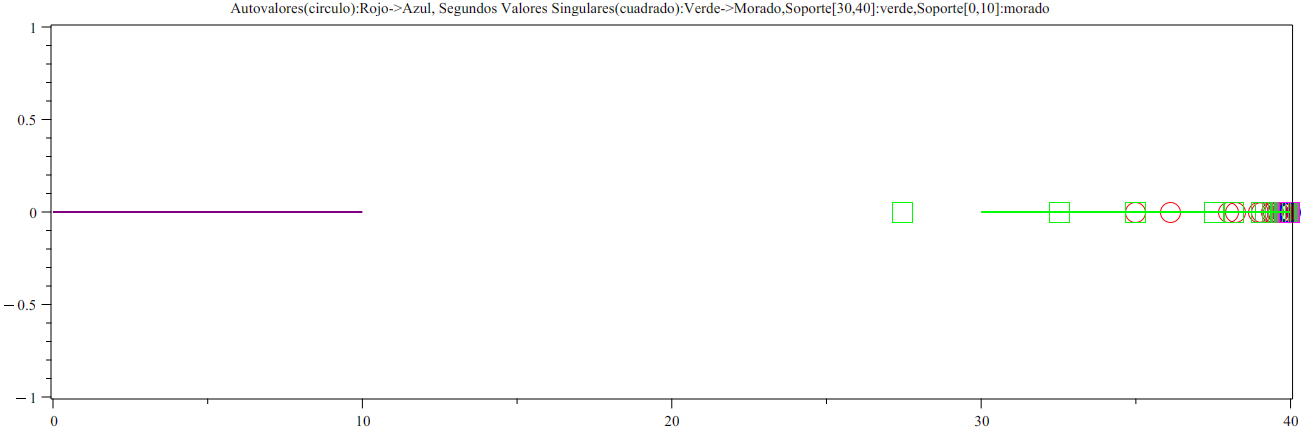
\includegraphics[width=1\textwidth]{include/a30b40c0d10.png}
\end{center}

\begin{enumerate}
	\item $\lim_{n \to 50}\sigma_{1,n}=\infty$
	\item $\lim_{n \to 50} \rho(\mathcal{D}_{n})=39.983$
	\item $\max\{\rho(\mathcal{D}_{n})\}_{n=0}^{50}=39.983$
	\item $\lim_{n \to 50}\sigma_{2,n}=39.982$
\end{enumerate}

\textbf{Ejemplo 5.}
$\langle p(t),q(t) \rangle_{\textbf{M}_S}=\int_{0}^{10} p(t)q(t) \, dt + \int_{30}^{50} p'(t)q'(t) \, dt $

\begin{center}
	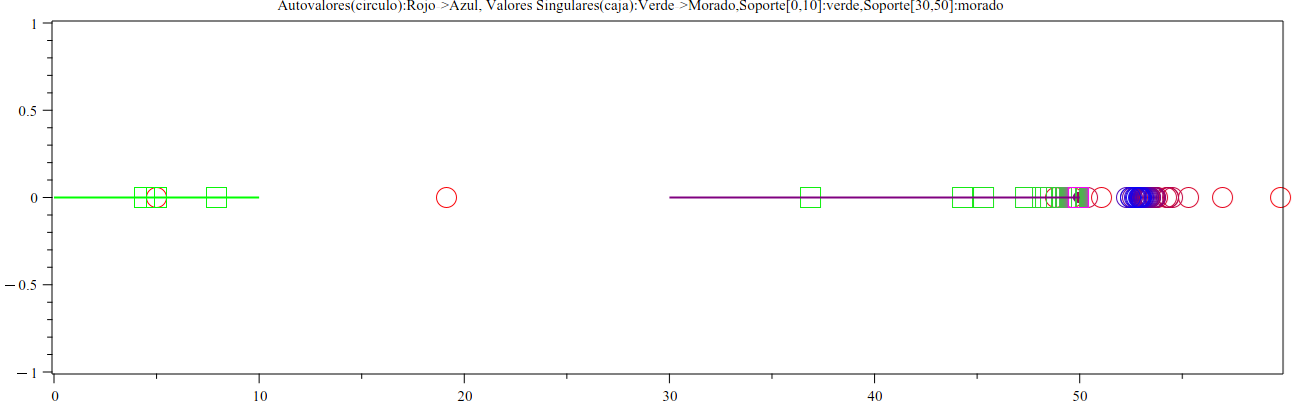
\includegraphics[width=1\textwidth]{include/a0b10c30d50.png}
\end{center}

\begin{enumerate}
	\item $\lim_{n \to 50}\sigma_{1,n}=\infty$
	\item $\lim_{n \to 50} \rho(\mathcal{D}_{n})=52.763$
	\item $\max\{\rho(\mathcal{D}_{n})\}_{n=0}^{50}=59.814$
	\item $\lim_{n \to 50}\sigma_{2,n}=49.966$
\end{enumerate}

\textbf{Ejemplo 6.}
$\langle p(t),q(t) \rangle_{\textbf{M}_S}=\int_{30}^{50} p(t)q(t) \, dt + \int_{0}^{10} p'(t)q'(t) \, dt $

\begin{center}
	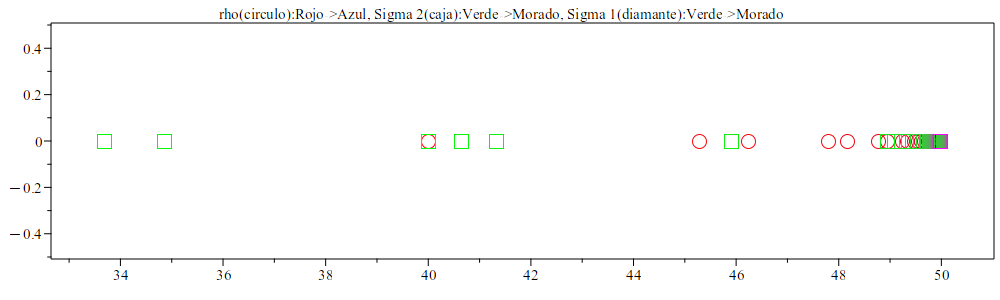
\includegraphics[width=1\textwidth]{include/a30b50c0d10.png}
\end{center}

\begin{enumerate}
	\item $\lim_{n \to 50}\sigma_{1,n}=\infty$
	\item $\lim_{n \to 50} \rho(\mathcal{D}_{n})=49.975$
	\item $\max\{\rho(\mathcal{D}_{n})\}_{n=0}^{50}=49.975$
	\item $\lim_{n \to 50}\sigma_{2,n}=49.975$
\end{enumerate}

\textbf{Ejemplo 7.}
$\langle p(t),q(t) \rangle_{\textbf{M}_S}=\int_{0}^{20} p(t)q(t) \, dt + \int_{30}^{40} p'(t)q'(t) \, dt $

\begin{center}
	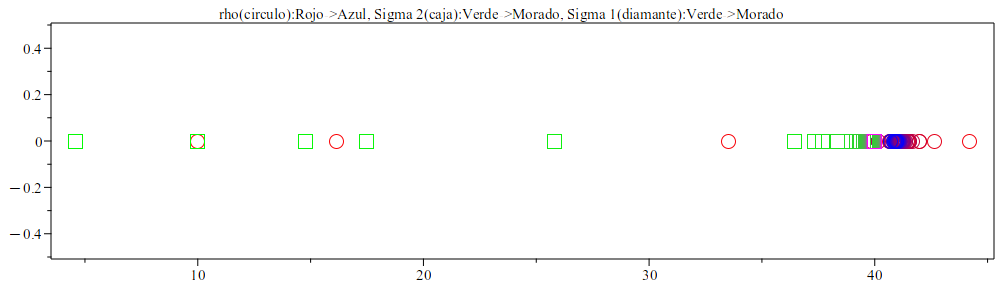
\includegraphics[width=1\textwidth]{include/a0b20c30d40.png}
\end{center}

\begin{enumerate}
	\item $\lim_{n \to 50}\sigma_{1,n}=\infty$
	\item $\lim_{n \to 50} \rho(\mathcal{D}_{n})=41.066$
	\item $\max\{\rho(\mathcal{D}_{n})\}_{n=0}^{50}=44.196$
	\item $\lim_{n \to 50}\sigma_{2,n}=39.970$
\end{enumerate}

\textbf{Ejemplo 8.}
$\langle p(t),q(t) \rangle_{\textbf{M}_S}=\int_{30}^{40} p(t)q(t) \, dt + \int_{0}^{20} p'(t)q'(t) \, dt $

\begin{center}
	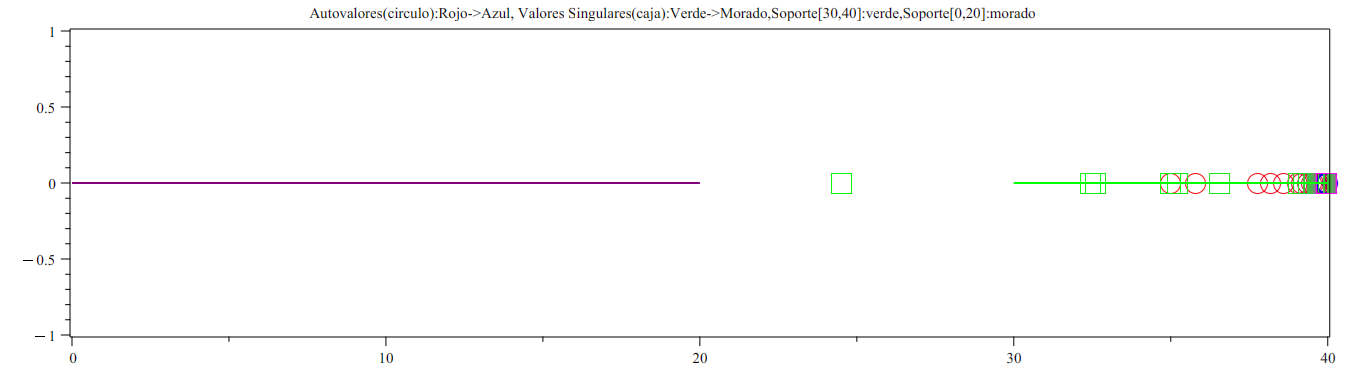
\includegraphics[width=1\textwidth]{include/a30b40c0d20.png}
\end{center}

\begin{enumerate}
	\item $\lim_{n \to 50}\sigma_{1,n}=\infty$
	\item $\lim_{n \to 50} \rho(\mathcal{D}_{n})=39.979$
	\item $\max\{\rho(\mathcal{D}_{n})\}_{n=0}^{50}=39.979$
	\item $\lim_{n \to 50}\sigma_{2,n}=39.979$
\end{enumerate}

\textbf{Ejemplo 9.}
$\langle p(t),q(t) \rangle_{\textbf{M}_S}=\int_{-15}^{-5} p(t)q(t) \, dt + \int_{5}^{16} p'(t)q'(t) \, dt $

\begin{center}
	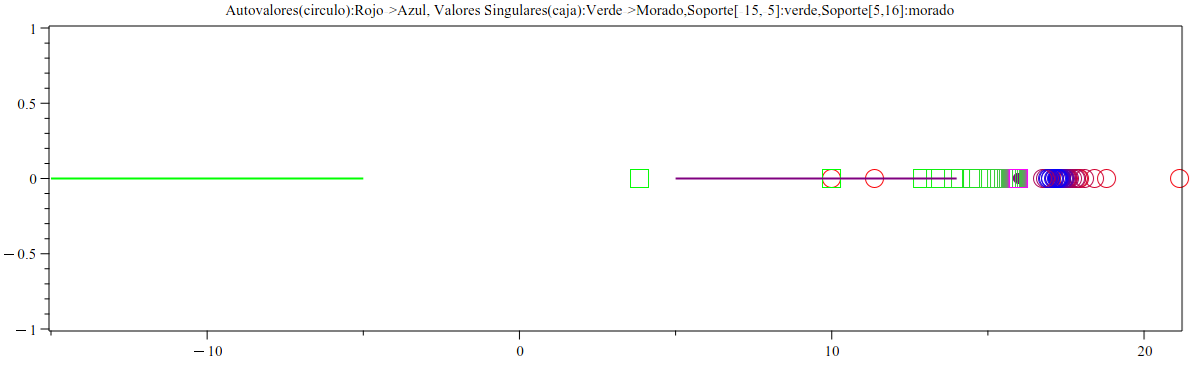
\includegraphics[width=1\textwidth]{include/a-15b-5c5d16.png}
\end{center}

\begin{enumerate}
	\item $\lim_{n \to 50}\sigma_{1,n}=\infty$
	\item $\lim_{n \to 50} \rho(\mathcal{D}_{n})=17.104$
	\item $\max\{\rho(\mathcal{D}_{n})\}_{n=0}^{50}=21.152$
	\item $\lim_{n \to 50}\sigma_{2,n}=15.980$
\end{enumerate}

\textbf{Ejemplo 10.}
$\langle p(t),q(t) \rangle_{\textbf{M}_S}=\int_{-15}^{-5} p(t)q(t) \, dt + \int_{5}^{14} p'(t)q'(t) \, dt $

\begin{center}
	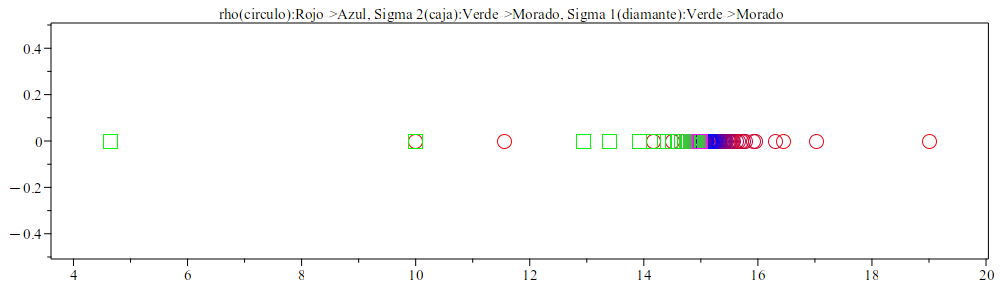
\includegraphics[width=1\textwidth]{include/a-15b-5c5d14.png}
\end{center}

\begin{enumerate}
	\item $\lim_{n \to 50}\sigma_{1,n}=\infty$
	\item $\lim_{n \to 50} \rho(\mathcal{D}_{n})=15.005$
	\item $\max\{\rho(\mathcal{D}_{n})\}_{n=0}^{50}=19.007$
	\item $\lim_{n \to 50}\sigma_{2,n}=14.985$
\end{enumerate}

Tras ver todos los ejemplos podemos conjeturar lo siguiente:\todo{lo que es claro es que lo que suceda con los soportes influye mucho, ya sea tamaño, extremos o intersección.}
\begin{itemize}
	\item El segundo mayor valor singular de $\mathcal{D}_{n}$ converge al extremo con mayor módulo de los soportes. Se puede encontrar una constante de proporción o de desviacion $K$ que depende de los soportes (extremos,intersección, tamaño) para poder acotar los ceros.\todo{puede que la k y K esten relacionadas}
	\item $\lim_{n \to \infty} \max{Z_n}=\max\{|a|,|b|,|c|,|d|\} + k = \max\{|a|,|b|,|c|,|d|\} \cdot k'$
	\item El $k$ cuando $\max\{|a|,|b|\} < \max\{|c|,|d|\}$ es notablemente mayor que el $k$ cuando ocurre lo contrario.
	\item $k$ o $k'$ depende de la posición relativa entre los soportes.
	      \begin{itemize}
		      \item Si $[a,b] \cap [c,d] = \emptyset$ y $dist(b,c) < dist(a,b) + dist(c,d)$ entonces $k$ o $k'$ no crece mucho.
		      \item Si $[a,b] \cap [c,d] = \emptyset$ y $dist(b,c) > dist(a,b) + dist(c,d)$ entonces $k$ o $k'$ crece mucho.
		      \item Si $[a,b] \cap [c,d] \neq \emptyset$ entonces $k$ o $k'$ crece muy poco. Mientras mayor sea $dist(b,c)$ menos crece $k$ o $k'$.
	      \end{itemize}
\end{itemize}
\todo{Tengo que hacer mas pruebas porque con tantos casos termina confundiendo que es lo que pasa.}

Dejando de lado los productos de Sobolev, consideremos el producto interno de la forma:
$$\langle p(t),q(t) \rangle = \int_{a}^{b} p(t) q(t) \, dt + |p'(c)||q'(c)|.$$
Este producto interno es muy interesante ya que solo introduce un átomo al producto interno usual, y sin embargo el operador multiplicación no es acotado. En los siguientes ejemplos se mostrará que los ceros de los polinomios ortogonales asociados a este producto interno están acotados, y que podemos encontrar una cota.

\textbf{Ejemplo 11.} $\langle p(t),q(t) \rangle = \int_{-1}^{1} p(t) q(t) \, dt + |p'(0)||q'(0)|.$

\begin{center}
	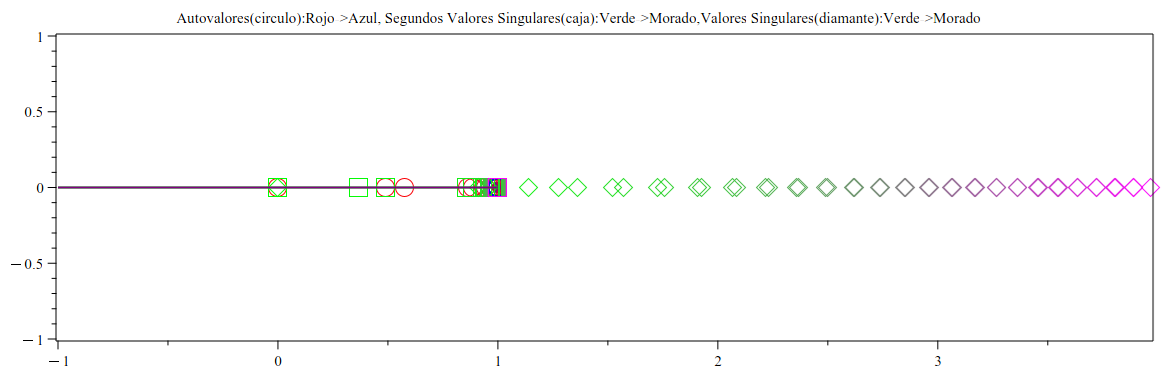
\includegraphics[width=1\textwidth]{include/a-1b1t0.png}
\end{center}

\begin{enumerate}
	\item $\lim_{n \to 50}\sigma_{1,n}=\infty$ (para $\mathcal{D}_{50}=3.971$)
	\item $\lim_{n \to 50} \rho(\mathcal{D}_{n})=0.999$
	\item $\max\{\rho(\mathcal{D}_{n})\}_{n=0}^{50}=0.999$
	\item $\lim_{n \to 50}\sigma_{2,n}=0.999$
\end{enumerate}

\textbf{Ejemplo 12.} $\langle p(t),q(t) \rangle = \int_{-1}^{1} p(t) q(t) \, dt + |p'(2)||q'(2)|.$

\begin{center}
	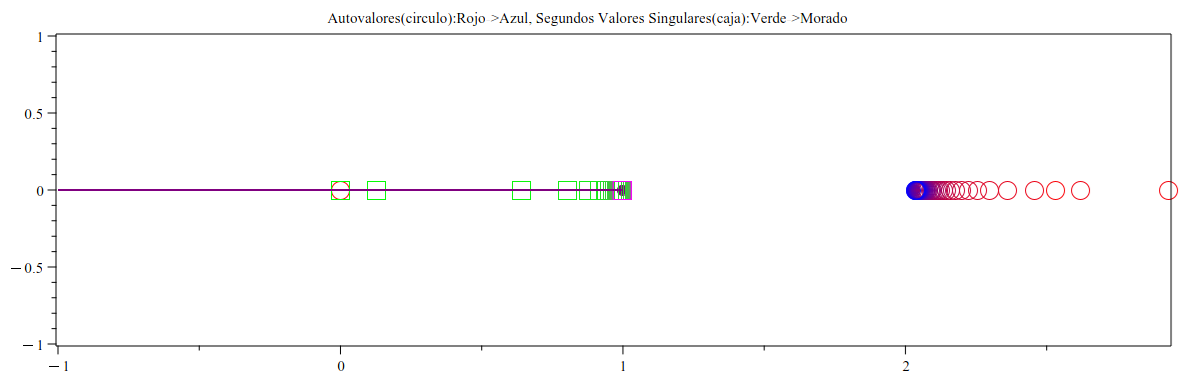
\includegraphics[width=1\textwidth]{include/a-1b1t2.png}
\end{center}

\begin{enumerate}
	\item $\lim_{n \to 50}\sigma_{1,n}=\infty$
	\item $\lim_{n \to 50} \rho(\mathcal{D}_{n})=2.0356$
	\item $\max\{\rho(\mathcal{D}_{n})\}_{n=0}^{50}=2.933$
	\item $\lim_{n \to 50}\sigma_{2,n}=0.999$
\end{enumerate}

\textbf{Ejemplo 13.} $\langle p(t),q(t) \rangle = \int_{0}^{1} p(t) q(t) \, dt + |p'(0)||q'(0)|.$

\begin{center}
	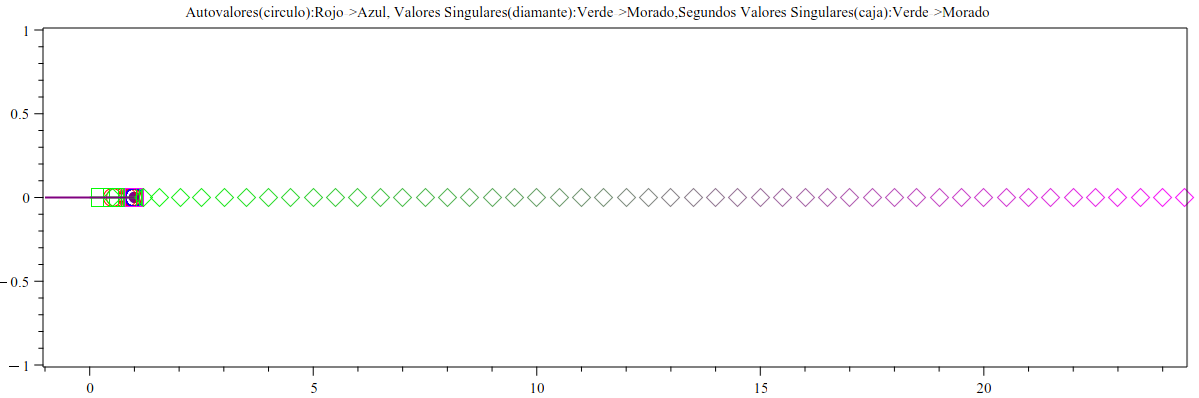
\includegraphics[width=1\textwidth]{include/a0b1t0.png}
\end{center}

\begin{enumerate}
	\item $\lim_{n \to 50}\sigma_{1,n}=\infty$ (para $\mathcal{D}_{50}=25.000$)
	\item $\lim_{n \to 50} \rho(\mathcal{D}_{n})=0.999$
	\item $\max\{\rho(\mathcal{D}_{n})\}_{n=0}^{50}=0.999$
	\item $\lim_{n \to 50}\sigma_{2,n}=0.999$
\end{enumerate}

\textbf{Ejemplo 14.} $\langle p(t),q(t) \rangle = \int_{0}^{1} p(t) q(t) \, dt + |p'(2)||q'(2)|.$

\begin{center}
	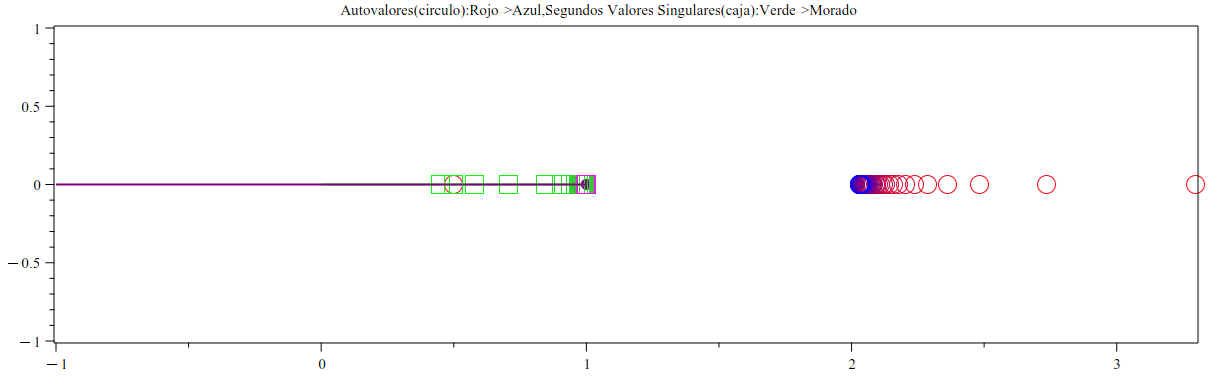
\includegraphics[width=1\textwidth]{include/a0b1t2.png}
\end{center}

\begin{enumerate}
	\item $\lim_{n \to 50}\sigma_{1,n}=\infty$
	\item $\lim_{n \to 50} \rho(\mathcal{D}_{n})=2.029$
	\item $\max\{\rho(\mathcal{D}_{n})\}_{n=0}^{50}=3.299$
	\item $\lim_{n \to 50}\sigma_{2,n}=0.999$
\end{enumerate}

A raíz de estos ejemplos podemos conjeturar lo siguiente:

\begin{itemize}
	\item Si $c \in [a,b]$ entonces los ceros convergen al límite del soporte, y podemos usar el segundo mayor valor singular como cota.
	\item Si $c \notin [a,b]$ entonces los ceros convergen al átomo, y podemos usar el átomo como cota. Pero necesitamos determinar el coeficiente $k$ para poder abarcar todos los ceros.\todo{intuyo que tambien va a tener que ver con la posición relativa entre el soporte y el átomo, y posiblemente el tamaño del soporte.}
\end{itemize}

\begin{sidewaystable}
	\centering
	\small
	\caption{Resumen de ejemplos sobre la localización de ceros.}
	\begin{tabular}{|c|cccc|cccc|cccc|}
		\hline
		\multirow{3}{*}{\textbf{Parámetros}}       & \multicolumn{4}{c|}{\textbf{SECUENCIALMENTE}} & \multicolumn{4}{c|}{\textbf{NO SECUENCIALMENTE}} & \multicolumn{4}{c|}{\textbf{ÁTOMO}}                                                                                                                                                                    \\
		                                           & \multicolumn{4}{c|}{\textbf{DOMINADO}}        & \multicolumn{4}{c|}{\textbf{DOMINADO}}           & \multicolumn{4}{c|}{}                                                                                                                                                                                  \\
		\cline{2-13}
		                                           & $\sigma_{1,n}$                                & $\rho(\mathcal{D}_{n})$                          & $\max\rho$                          & $\sigma_{2,n}$ & $\sigma_{1,n}$ & $\rho(\mathcal{D}_{n})$ & $\max\rho$ & $\sigma_{2,n}$ & $\sigma_{1,n}$ & $\rho(\mathcal{D}_{n})$ & $\max\rho$ & $\sigma_{2,n}$ \\
		\hline
		\textbf{Ej.1}: $[-1,1]t^2, [-1,1]t^{10}$   & 1.276                                         & 0.999                                            & 1.133                               & -              & -              & -                       & -          & -              & -              & -                       & -          & -              \\
		\textbf{Ej.2}: $[-1,1]t^{10}, [-1,1]t^{2}$ & 2.204                                         & 0.999                                            & 1.275                               & -              & -              & -                       & -          & -              & -              & -                       & -          & -              \\
		\textbf{Ej.3}: $[0,10], [30,40]$           & -                                             & -                                                & -                                   & -              & $\infty$       & 43.133                  & 50.052     & 39.975         & -              & -                       & -          & -              \\
		\textbf{Ej.4}: $[30,40], [0,10]$           & -                                             & -                                                & -                                   & -              & $\infty$       & 39.983                  & 39.983     & 39.982         & -              & -                       & -          & -              \\
		\textbf{Ej.5}: $[0,10], [30,50]$           & -                                             & -                                                & -                                   & -              & $\infty$       & 52.763                  & 59.814     & 49.966         & -              & -                       & -          & -              \\
		\textbf{Ej.6}: $[30,50], [0,10]$           & -                                             & -                                                & -                                   & -              & $\infty$       & 49.975                  & 49.975     & 49.975         & -              & -                       & -          & -              \\
		\textbf{Ej.7}: $[0,20], [30,40]$           & -                                             & -                                                & -                                   & -              & $\infty$       & 41.066                  & 44.196     & 39.970         & -              & -                       & -          & -              \\
		\textbf{Ej.8}: $[30,40], [0,20]$           & -                                             & -                                                & -                                   & -              & $\infty$       & 39.979                  & 39.979     & 39.979         & -              & -                       & -          & -              \\
		\textbf{Ej.9}: $[-15,-5], [5,16]$          & -                                             & -                                                & -                                   & -              & $\infty$       & 17.104                  & 21.152     & 15.980         & -              & -                       & -          & -              \\
		\textbf{Ej.10}: $[-15,-5], [5,14]$         & -                                             & -                                                & -                                   & -              & $\infty$       & 15.005                  & 19.007     & 14.985         & -              & -                       & -          & -              \\
		\textbf{Ej.11}: $[-1,1], c=0$              & -                                             & -                                                & -                                   & -              & -              & -                       & -          & -              & $\infty$       & 0.999                   & 0.999      & 0.999          \\
		\textbf{Ej.12}: $[-1,1], c=2$              & -                                             & -                                                & -                                   & -              & -              & -                       & -          & -              & $\infty$       & 2.0356                  & 2.933      & 0.999          \\
		\textbf{Ej.13}: $[0,1], c=0$               & -                                             & -                                                & -                                   & -              & -              & -                       & -          & -              & $\infty$       & 0.999                   & 0.999      & 0.999          \\
		\textbf{Ej.14}: $[0,1], c=2$               & -                                             & -                                                & -                                   & -              & -              & -                       & -          & -              & $\infty$       & 2.029                   & 3.299      & 0.999          \\
		\hline
	\end{tabular}
\end{sidewaystable}